% vim: ft=tex
\chapter{Approach}
TODO what have we done to arrive at the goal (should be reproducible)\\
TODO this is probably what we know as "Concept"\\


\section{Getting familiar with Roadster}
The client gave a short introduction into Roadster's code base during the first
week of this thesis. Although quite overwhelming, the first impression was that
the code is clean, makes use of useful abstractions and has loosely coupled
classes. API documentation is scarce though.

TODO: describe approach of getting more familiar with Roadster, e.g. during prototyping

\section{Testing}
This section describes the test methods we used to check particular methods,
the integration of multiple components, as well as the behavior of the whole application.
All test resuts can be found in \autoref{ch:res}.

\subsection{Setup}
Due to the fact that Roadster's Github repository is private, online \gls{CI}
services such as \emph{Travis
CI}\footnote{url{https://travis-ci.com/}} can't be used without
payment\footnote{Payment is required after the first 100 builds.}. Fortunately,
Gitlab CI is free and can be installed on one's own infrastructure, such as the
\gls{VM} provided by HSR, where it was installed and configured. Unit and
integration tests are run every time new commits are checked in. This is useful
to get informed proactively when something breaks.

\subsection{Unit tests}
To ensure the correctness of the implementations, unit tests are written using
RSpec. 100\% coverage of the students' contributions can be achieved by
adhering to \gls{TDD}. Naturally, this also simplifies refactoring the code
without risking things breaking silently. Unit tests reside under the \sh{spec}
directory of Roadster's code base.

\subsection{Integration tests}
Integration tests verify the interaction between the individual components.
To test core features like cluster, high availability, and persistence
synchronization, integration tests have been written. Multiple nodes can be
simulated easily by starting them as different process groups. This is possible
since \zmq completely abstracts the transport away.

In order to test the failover or synchronization functionality, individual processes
can simply be killed and restarted later if the scenario defines this.

More details about the integration test scenarios can be found in \autoref{ch:res}.

\subsection{Continous integration}
\gls{CI} helps us prevent integration problems also known as \emph{integration
hell}. Each push to the repository will trigger a CI check, which will run a
build script. This will install Roadster's dependencies, an example app built
with Roadster, and finally Roadster's test suites.

\subsection{System test}
Systemtests dienen dazu die Applikation unter realen Bediengungen zu testen. Um eine fast realitätsnah
Umgebung zu erschaffen, kam mininet, jnettop und fake SPS Steuerungen zum Einsatz.
\begin{description}
	\item [Mininet:]
		Mininet erlaubt es adhoc VirtuelMachine's zu starten, 
		welche einen gemeinsamen Kernel teilen.
		Dies ermöglicht es auf einem Rechner viele Nodes/Rechner zu starten. 
		Mittels mininet können auch Verbindungen zwischen Nodes getrennt werden
		um Netzwerkprobleme zu simulieren. 
	\item [jnettop:]
		jnettop simuliert Netzkapazitätprobleme auf den einzelnen Verbindungen.
	\item [fake sps:]
		Fake SPS Steuerungen sind einfache Scripts, welche auf Anfragen antworten.
\end{description}

Alle Ereignise wurden in Logdateien gespeichert, welche für die Auswertung des Ergebnis gebraucht wurden. 
Mit einem Ruby Programm wurden diese Logdateien auf korrektheit überprüft.
Alle Systemtests wurden manuell nach jeder construction phase ausgeführt.\\
\\
System tests are designed to test the application under real conditions. 
To create an almost realistic environment we used mininet, jnettop and fake \gls{PLC} controls for deployment.
\begin{description}
	\item [Mininet:]
		Mininet allows adhoc start VirtuelMachine's, which share a common kernel.
		This makes it possible on a computer to start many nodes / hosts. 
		Mininet can also simulated connection problems between nodes.
	\item [jnettop:]
		jnettop simulated network capacity problems on the individual network connections between the nodes.
	\item [fake sps:]
		Fake \gls{PLC} controls are simple scripts that respond to requests.
\end{description}

All events were stored in log files, which were used for the evaluation of the result. 
A Ruby program checked these log files on correctness. All system tests were performed manually 
after each construction iteration.

\subsubsection{Test scenarios}
Die Testszenarien enthalten primär nur mögliche Bediengungen wie sie in einer realen Situation anzutreffen sind. Aus wissenschaftlichen Interesse wurden weitere Szenarien
getestet, welche den Extremfall abbilden sollten.\\
\\
The test scenarios only includes possible combinations as they are encountered in a real situation. From scientific interest
we added more test scenarios, which reflected the extreme cases.
\begin{description}
	\item [ML-HA:]
		Multi Layer mit zwei ebenen. Die erste Ebene enthält ein Node, 
		welches die Steuerungen überwacht. Die zweite Eben hat einen Primary und Backup.
	\\TODO ...
	\item [SL-HA:]
		Single Layer. Ein Primay und Backup Node welche beide direkt mit der Steuerungen verbunden sind.
		\\TODO ...
\end{description}
Persistence wird bei allen Tests mit geprüft, da sie zu Non functional requirements gehört und bei allen Szenarien aktiv ist.
\\TODO Extremfall ... 3 Ebenen mit 1 ebe
\\
Testszenarien enthalten die Konfiguration von Mininet und den einzelnen Nodes. 
Der Ablauf der Szenarios wurde im Detail beschrieben um die Ergebnisse reproduzierbar zu machen.


TODO work out methodology (maybe with mininet, shell scripts, and analyze logs retrospectively)\\
TODO integration tests at the end of every iteration\\
TODO system tests at end of construction\\
TODO use travis-ci.com OR GitLab CI (self-hosted on HSR VM)\\

%----------------------------------------------------------------------------
\section{Port to new \zmq library}\label{sec:meth:port}
Porting Roadster to a new \zmq library early on makes sense for the following reasons:

\begin{itemize}
\item to exclude possible failures from faults in the unmaintained ffi-rzmq\footnote{\url{https://github.com/chuckremes/ffi-rzmq}} library
\item encryption is needed later anyway, which is not supported by the currently used library
\item all other tasks involve \zmq communication anyway
\end{itemize}

There is currently only a single Ruby library that is maintained, supports
encryption, and freely available, which is \gls{cztop}. Technically it's a
binding for the \gls{czmq} library, which is the modern and recommended way of
using \zmq. More info about CZMQ can be found in \autoref{ch:zmq}.

As stated in the Task Description already, Roadster's event loop makes use of
the \zmq options \sh{ZMQ_FD} and \sh{ZMQ_EVENTS}. Getters for these had to be
added to in CZTop, which was a matter of minutes.

\subsection{Actual port}
Due to Roadster's beautiful software architecture, code that actually made use
of the ffi-rzmq library directly was located in a single file. The following
things needed to be done:

\begin{itemize}
\item Tell Ruby to load CZTop instead of ffi-rzmq.
\item Remove code to send and receive multi-part messages. This has been simplified
in CZMQ and thus is a single method call using CZTop.
\item Remove error checking code. CZTop always checks error codes, and raises
an appropriate exception if needed.
\item Simplify code that reads option values such as \sh{ZMQ_FD} and \sh{ZMQ_EVENTS}.
\item Rewrite library calls to use CZTop instead of ffi-rzmq.
\end{itemize}

This was about an hour's work.

%----------------------------------------------------------------------------
\section{Cluster}\label{sec:meth:cluster}
A Roadster cluster is illustrated in \autoref{fig:cluster}. Adding cluster
functionality to Roadster involves the following aspects:
\begin{itemize}
	\item node topology DSL

		This DSL also has to provide means to define the roles/functionality of each node, e.g. the set of COMM actors running on a particular node

	\item DIM synchronization
	\item message routing
	\item What needs to be done if a WebUI user wants to e.g. change some value on a PLC, possibly on a remote node? Is it completely handled via DIM or do we need message routing?
\end{itemize}

\begin{figure}[]
	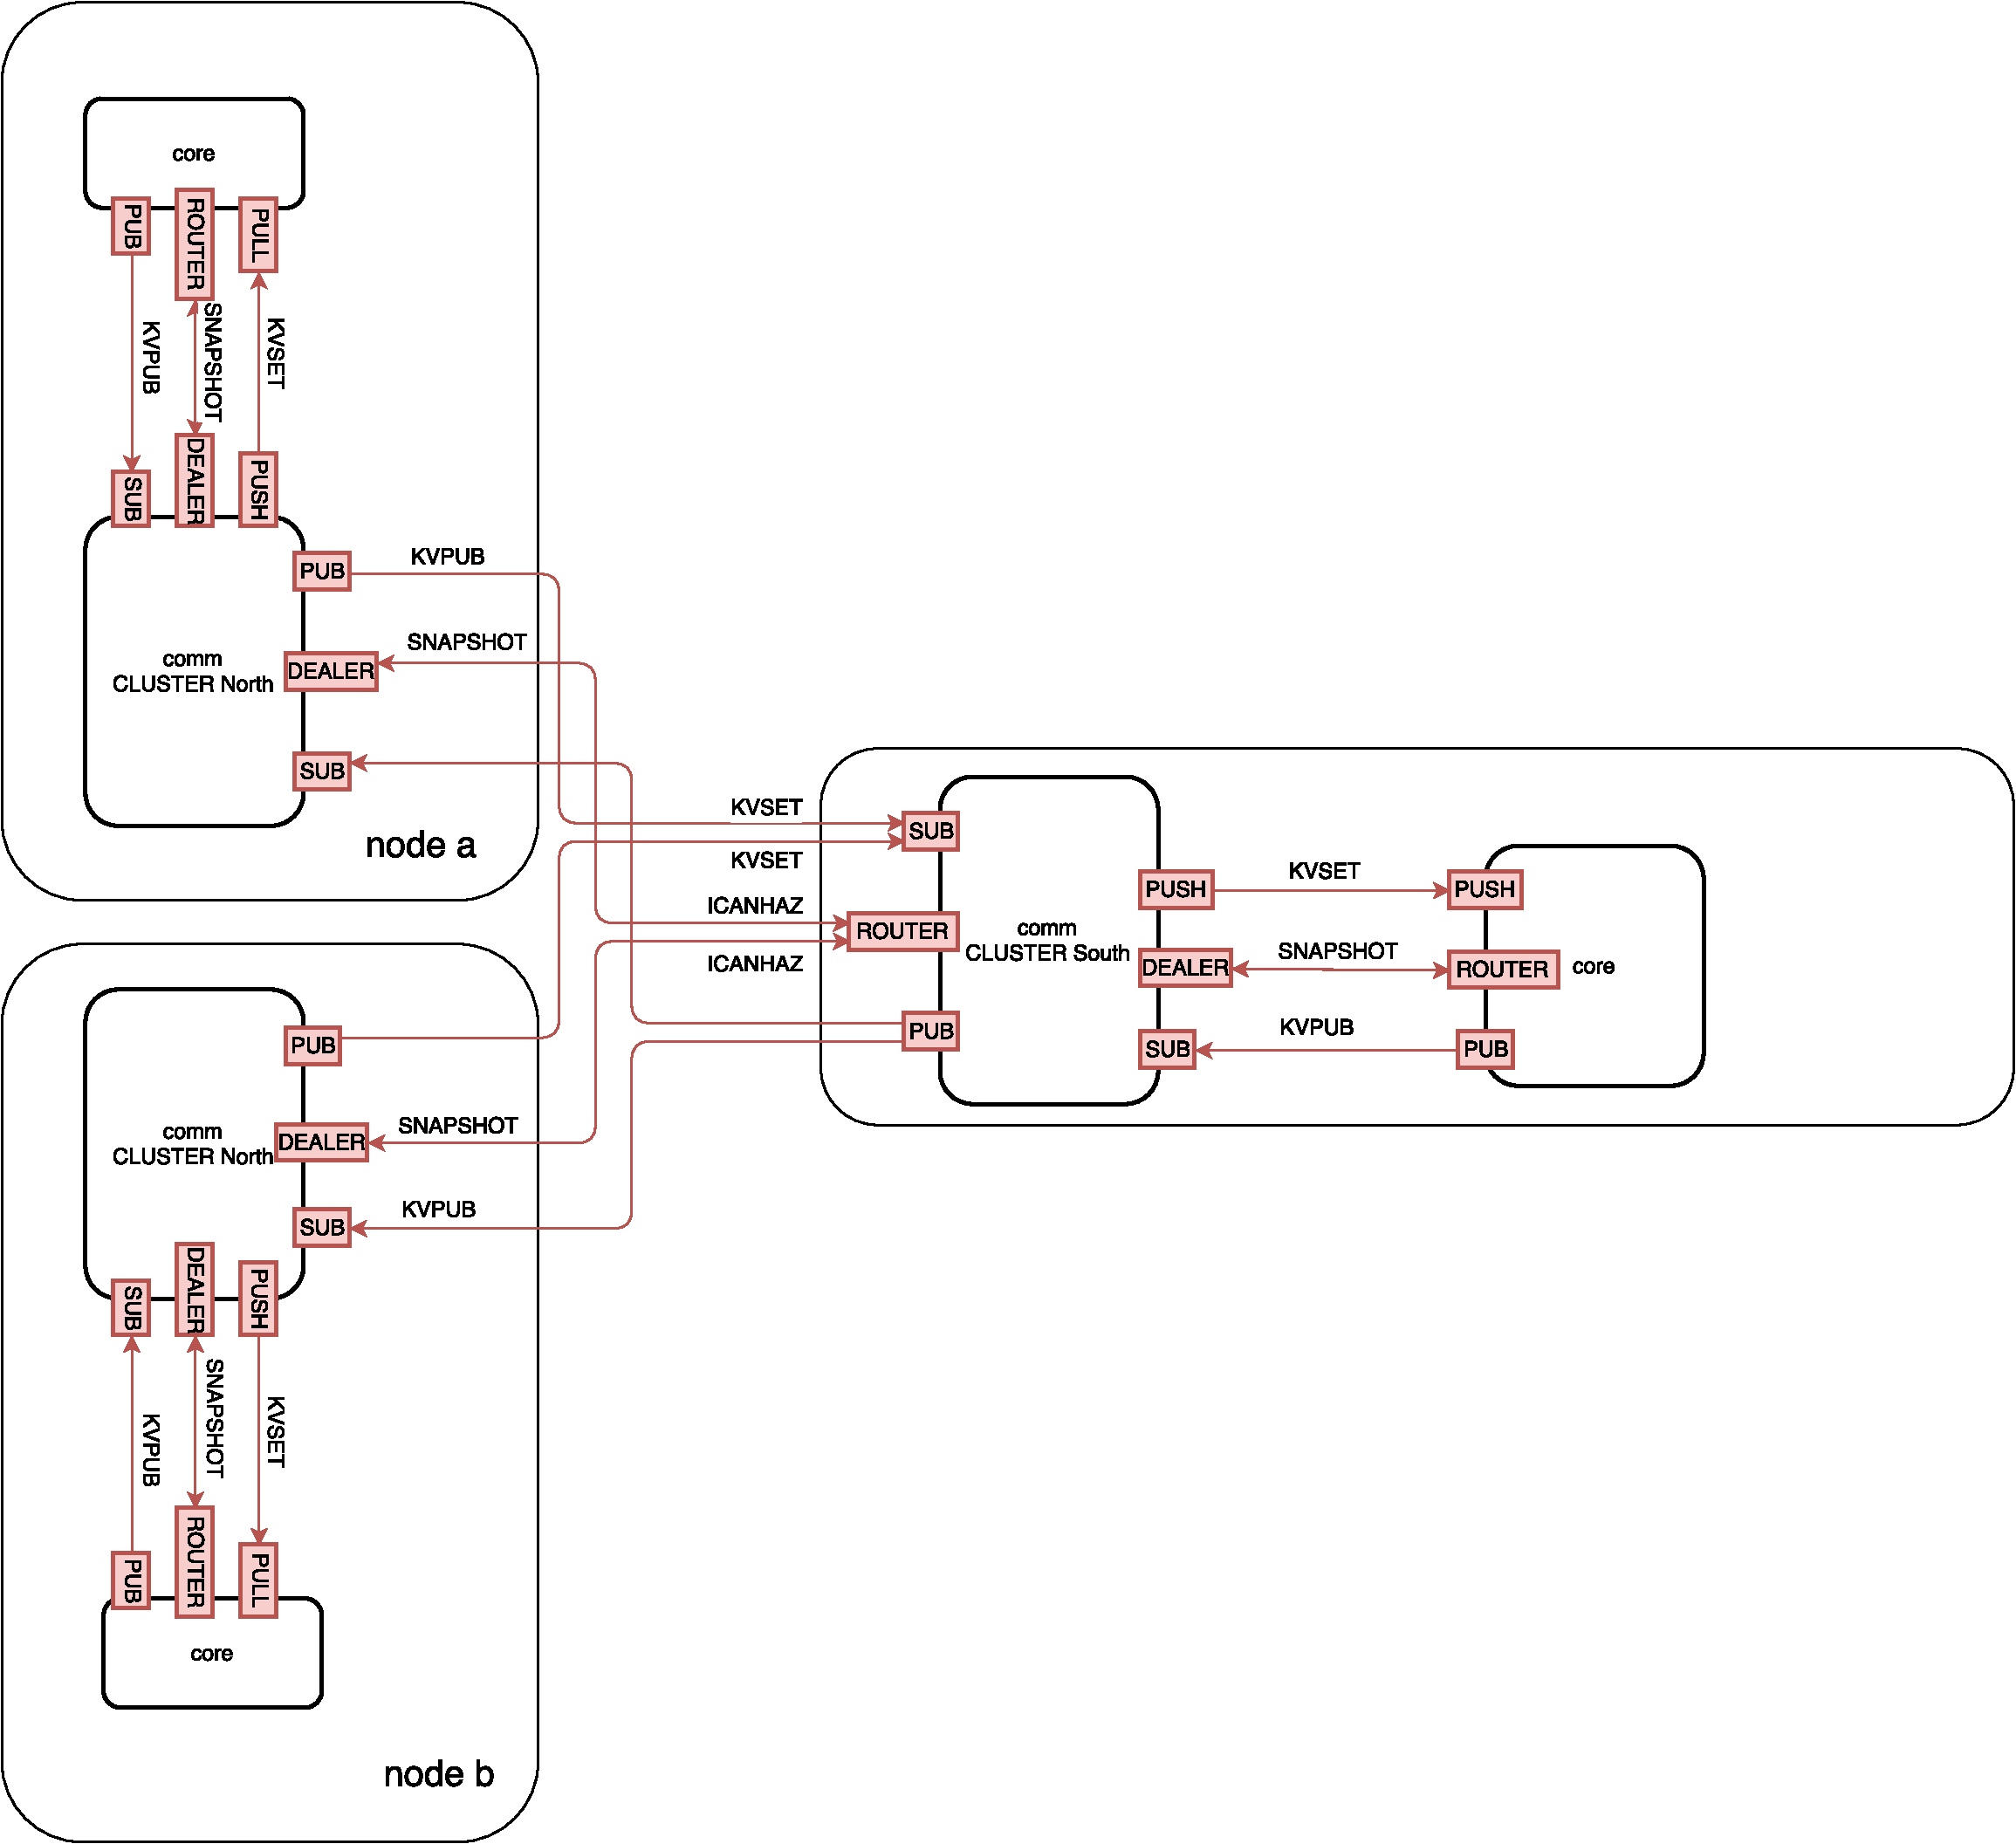
\includegraphics[width=\textwidth]{img/cluster_protocol.pdf}
	\caption{Cluster setup between a supernode and two subnodes}
	\label{fig:cluster}
\end{figure}

\subsubsection{Fallacies of Distributed Computing}
At this place, it is worth noting the common fallacies encountered in
distributed computing, as explained on \cite{dcomp:fallacies}.

\subsection{DIM Synchronization}
The following is a list of things that are missing before the requirements can be fulfilled:
\begin{itemize}
\item it has to work across several nodes
\item it has to be able to handle HA supernodes, which affects DIM synchronization and message routing
\end{itemize}

There are multiple choices when it comes to what exactly of the DIM should be synchronized:

\begin{description}
	\item [Variant 1. Sync self-subtree only:] \hfill
		\begin{itemize}
			\item always sync on self-subtree only
			\item con: no copy of remaining tree
		\end{itemize}

	\item [Variant 2. Sync complete tree:] \hfill
		\begin{itemize}
			\item always sync on complete tree
			\item get snapshot and merge own subtree
		\end{itemize}

	\item [Variant 3. Either sync on subtree or complete tree:] \hfill
		\begin{itemize}
			\item make it configurable: either sync on subtree or complete tree
		\end{itemize}
\end{description}

Variant 2 will be the first step. Variant 3 will be the second step, if at all.

Since COMM actors are used to communicate with things outside of a node, new COMM
actors will have to be introduced: One kind that is south-facing to communicate
with subnodes, and another one that is north-facing for communication with
supernodes. They will be named COMM CLUSTER NORTH and COMM CLUSTER SOUTH.

Their responsibility is the inter-node synchronization of the DIM, similarly to
what's happening in the existing CSP within a single node.

To send KVSET updates from one actor to the CORE actor, PUSH-PULL sockets are
used. However, similar to the \gls{CHP} described in the \gls{zguide}, this
mechanism here needs to be able to handle replication to one or two (in case of
HA) superordinate nodes. That means using PUB-SUB messaging for is more
appropriate, so all direct superordinate nodes hear the updates.

\subsubsection{CAP theorem}
The CAP theorem \cite{wp:cap} states that it is impossible for a distributed
computer system to simultaneously provide consistency, availability, and
network partition tolerance. In the face of a network partition, one has to
chose between availability and consistency. Because sub trees of a Roadster
cluster must be autonomous, availability is chosen.

Eventual consistency is guaranteed by restricting write access to the owning
node, and recovering from a network partition when communication is restored is
done by simply reinitiating the DIM synchronization process.

\subsection{Node Typology Definition}
A cluster's node topology has to be defined somewhere. This can be done using a
\gls{DSL} and then put into a static file (e.g. \sh{topology_conf.rb}) shared
on all nodes of a Roadster cluster. Each actor could then read the file at
startup, just like it's done for other configuration pieces of a Roadster node.
\autoref{lst:dsl:topo:no-ha} shows how such a configuration snippet might look.

To let the actors of a node know which node they belong to, an additoinal line
has to be added to the specific configuration file (\sh{conf.rb}), e.g.
\rb{conf.system_id = "nodes.root"}. Using that information, the topology
created using the DSL can be walked like a tree to find the correct node and
important information like its neighbor nodes.

A HA node pair could be one DIM object which has one name but two IP addresses
(primary and backup, in that order). Direct subnodes can use that information
to connect to the correct superordinate node during normal operation and also
when the primary node is unavailable. The respective DSL snippet is shown in
\autoref{lst:dsl:topo:with-ha}.

Not every node in a cluster is the same: Some are only connected with other
nodes, some also talk to field devices. To define different node roles, a
syntax as shown in \autoref{lst:dsl:topo:with-roles} is possible.

\begin{lstlisting}[style=customruby,caption={Cluster DSL example without HA}, label={lst:dsl:topo:no-ha}]
# * basic method to add a node: #add_node(ID, south_facing_bind_endpoint)
# * it takes a block for defining subnodes

conf.nodes do |map|
  map.add_node("root", "tcp://10.0.0.1:5000") do |map|
    map.add_node("subnode_a", "tcp://10.0.0.10:5000")
    map.add_node("subnode_b", "tcp://10.0.0.11:5000")
  end
end

# subnode_a can infer its endpoints from its position in the tree:
conf.system_id = "nodes.root.subnode_a"
#=> this node is "subnode_a"
#=> its IP address is 10.0.0.10
#=> north facing COMM actor's bind port is 5001
#=> south facing COMM actor's bind port is 5000
#=> north facing COMM actor will connect to "root" node on "tcp://10.0.0.1:5000"
\end{lstlisting}

\begin{lstlisting}[style=customruby, caption={Cluster DSL example with HA}, label={lst:dsl:topo:with-ha}]
conf.nodes do |map|
  map.add_ha_pair("root", "tcp://10.0.0.1:5000", "tcp://10.0.0.2:5000") do |map|
    map.add_node("subnode_a", "tcp://10.0.0.10:5000")
    map.add_node("subnode_b", "tcp://10.0.0.11:5000")
  end
end

# subnodeA can infer its endpoints from its position in the tree:
conf.system_id = "nodes.root.subnode_a"
#=> this node is "subnode_a"
#=> its IP address is 10.0.0.10
#=> north facing COMM actor's bind port is 5001
#=> south facing COMM actor's bind port is 5000
#=> north facing COMM actor will connect to "root" HA pair on "tcp://10.0.0.1:5000" OR "tcp://10.0.0.2:5000" (Lazy Pirate algorithm)

# for primary root:
conf.system_id = "nodes.root[primary]"
\end{lstlisting}

% ############
% # within ba-roadster-app's lib/domain/domain.rb file:
% #
\begin{lstlisting}[style=customruby, caption={Cluster DSL example with HA and roles}, label={lst:dsl:topo:with-roles}]
# Idea for node topology definition and assigning roles (features/adapters) to
# diffent kinds of nodes.

module Roadster
  module Domain::Model

    build do
      nodes do
        node "root" do # or maybe ha_node or bstar_node
          endpoint "tcp://10.0.0.1:5000", "tcp://10.0.0.2:5000"
          label 'BA Roadster App'
          desc  'Sample application for experimenting and developing the new features within the scope of the Bacherlor Thesis of Patrik Wenger and Manuel Schuler at HSR.'

          load_conf ::Conf::AccessControl
          load_conf ::Conf::Objects
          load_conf ::Conf::Navigation

          node "subnode_a" do
            endpoint "tcp://10.0.0.1:5000"
            load_conf ::Conf::Adapters
            # load_conf ...
          end
        end
    end

  end # Domain::Model
end # Roadster
\end{lstlisting}


\subsection{Message Routing}
Messages need to be sent from an actor on one node to an actor on another node. The best place to put this logic is the CORE actor which already does this for messages exchanged within a node. It needs to be extended to know about nodes and their actors, not only actors on the current node. Then messages can be passed around hop-by-hop.

In case a message is sent in \emph{Dialog} mode, this implicates Russian doll routing: At every hop, a new dialog is started which expects an immediate response, which will subsequently be passed back and complete the open dialogs.

\subsubsection{Example}
When a user of the root node's web UI wants to change a value on a field device
connected to the root node's subordinate node, a command is sent from the
browser to the web UI's COMM actor. From there it's sent via the CORE actor out
on the south-facing CLUSTER actor to the subordinate node. There it's routed
via the CORE actor to the correct COMM actor, where the command can actually be
executed on the field device.

%----------------------------------------------------------------------------
\section{High Availability}\label{sec:meth:ha}
If Roadster is going to be run in a cluster setup, measures need to be taken to
mitigate the risk of failure, since many nodes are more likely to fail than a
single node (unless they add redundancy). Availability shall be ensured by
adding redundancy on certain levels of the node hierarchy (e.g. at the bottom
of the topology, right above the PLC, or at the root level), in the form of a
fully functional backup node in addition to the primary one.

Run together in a hot-standby cluster, the passive node's responsibility is to
take over in case the active one goes down.

\subsection{Defining Reliability}
When speaking about reliability, it's worth listing the failures we want to be
able to handle. According to the requirements, these are exactly:

\begin{description}
	\item [Hardware or software failure on the primary node:]
		This could be one of the actors crashing, the whole OS
		crashing, or a fatal disk failure, irrecoverable memory error,
		or even just someone accidentally pulling the power plug.

	\item [Network failure]
		This only includes the failure of the link connecting a HA node
		to the rest of the cluster.  Interestingly, this limitation applies to both
		single level and multi level HA.
\end{description}

Failures that won't be covered include:
\begin{description}
	\item [Failure of the link between a subnode one of its supernodes:]

		This can't be handled since the two HA peers would have to
		continually share the number of subnodes connected to them, and
		based on that, make a decision on which one should be active or
		passive. Since the link between them could fail as well, this
		decision can't be done reliably, which could lead to the
		dreaded split brain syndrome.

	\item [Failure of the link between a HA peer node and the PLC]
		The \gls{bstar} algorithm won't initiate a failover since the
		active is still alive and is able to tell the passive node so.
		The missing life signs via the PLC could cause an alarm, but no
		failover, since they're only half of the conditions that have
		to be met for a failover.
\end{description}

\subsection{What's Needed}
TODO A simple HA protocol: Binary Star\\
TODO maybe we need to extend binary star to handle other kinds of network failures?\\
TODO new actor: COMM BSTAR\\

\subsection{Binary Star in a Nutshell}
Two HA peer nodes are started either as primary or as backup. After an initial
handshake, the primary one becomes active, the backup node becomes passive. The
two continually exchange heartbeats. Clients always connect to the primary's endpoint first.

The passive node takes over when the following two conditions are met:

\begin{enumerate}
\item no life signs from the active node
\item connection requests from clients
\end{enumerate}

The second condition is to prevent the split-brain syndrome and thus can be
thought of as an external vote for the node to actually initiate the failover.
This works because clients will always try to connect to the primary node's
endpoint first, then move on to the backup node's endpoint. In the
\gls{zguide}, this algorithm is explained as the \emph{Lazy Pirate} pattern,
one of the \emph{Reliable Request-Reply Patterns}.

\subsection{Failover}
In case the currently active node goes down, the two conditions will be met.
This means that the passive node starts accepting snapshot requests (ICANHAZ
messages) and updates the DIM, so every other node will know about the new,
active node. This is needed for the message routing to work.

It's important to mention that a dedicated, direct link from one HA node to its
peer actually worsens high availability. In case the non-dedicated link from
the primary HA node goes down, meaning the HA node is effectively offline and
unavailable for subnodes, the failover won't happen since heartbeats are still
exchanged with the HA peer node over the dedicated link.

\subsubsection{Alarm Generation}
When a failover happens, we want to create a \rb{Case} (alarm) in the DIM, so
the outage is visible to a user in one of the web UIs. Also, in case the
passive node goes down, which doesn't have an immediate effect on availability,
we also want to create a \rb{Case}. This is so the user can act upon the alarm
and e.g. initiate field forces to inspect the failed node and repair it.

Once repaired, it's started with the exact same configuration (either primary
or backup) again. Since there's already an active node (either the primary one,
or the backup one), the newly repaired node will become the new passive node.

\subsubsection{Failover from Backup to Primary}
Once failed over, the newly actve backup node stays active. It does so until it
fails itself, at which point the now repaired, up and running primary node will
take over. This works because the \gls{bstar} operates symmetrically
after successful initialization. But it never automatically switches back to
make the primary node the new active one without a failure. This is key. If a
node goes down, the failover happens automatically, but anything else will
require human interaction.

\subsection{Side benefit: Rolling Upgrades}
TODO useful for upgrades (maybe in Discussion)\\

\subsection{Dangerous corner case: Backup node active, dedicated link goes down, and there are new/reconnecting clients}
TODO this will lead to split-brain syndrome (maybe in Discussion)\\
TODO in general: dedicated link for HA pair communication is dangerous!\\

\subsection{Single Level}
This is different from what's described in the zguide because the concept of
client requests is missing here (PLCs don't request anything).  What can be
done instead is periodically sending life signs from one node to the other
through the PLC by updating some designated memory block. This can actually be
done by both the active and the passive node, which reduces code complexity.

The passive node will check the active node's life signs periodically as well.
In case the life signs cease, it can give its vote to the COMM BSTAR actor.
This would satisfy the second condition of the \gls{bstar} for a
failover to take place. The first condition would be the missing heartbeats
which are normally transmitted through the network link.

TODO new actor: COMM PLCVOTER\\

\begin{figure}[!ht]
	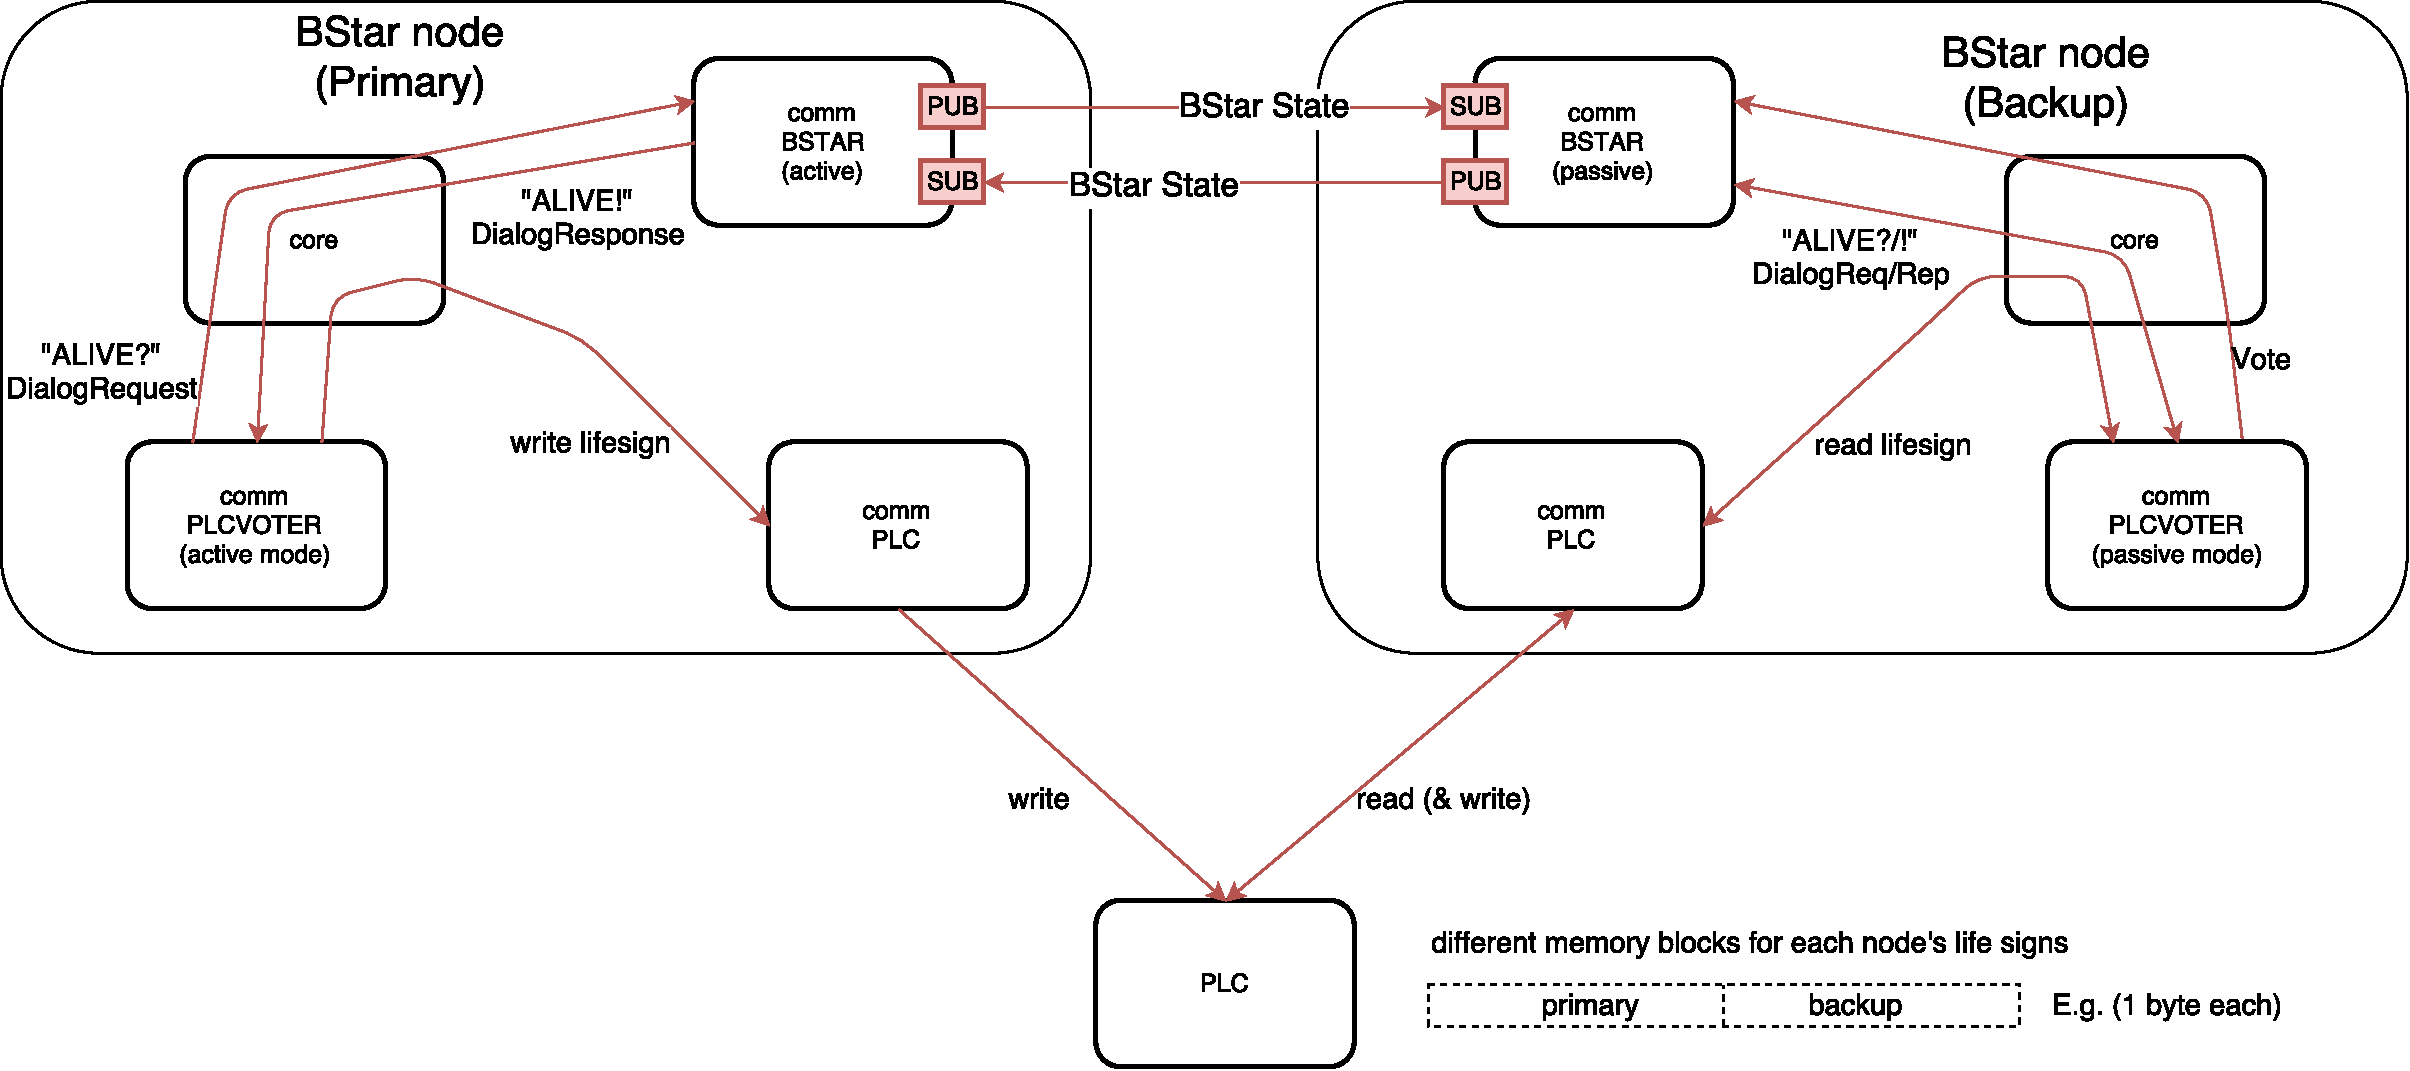
\includegraphics[width=\textwidth]{img/SL-HA_bstar.pdf}
	\caption{Single level HA setup between a HA pair and a PLC}
	\label{fig:sl-ha}
\end{figure}
% TODO: mention figure in text

\subsubsection{Caveats}
Special attention needs to be paid when it comes to writing these life signs. A
na\"ive developer might implement the COMM PLCVOTER so it autonomously causes
life signs to be written PLC. This works as long as the failures only affect
the hardware. But what if a software error happens in the CORE or BSTAR actor?
They'd crash or hang, while the PLCVOTER happily sends out life signs, which it
obviously shouldn't be doing at that moment.

A better implementation would have the PLCVOTER poll the BSTAR via the CORE
router whether it's still alive, and only send out a life sign in case it gets
an answer. This way, the BSTAR and the CORE actor are being tested for
responsiveness. We'll call the two messages being sent back and forth "DEAD?"
and "ALIVE!".

\subsubsection{Node---PLC Link Failure}
TODO describe why this won't cause a failover and thus can't be handled, as
mentioned above\\

\subsubsection{Supporting Different PLCs}
TODO: adapter

\subsection{Multi Level}
This kind of \gls{HA} setup is closely related to the \gls{bstar} described
in the \gls{zguide}, meaning that there will be actual requests from client on the
passive node in case the active node fails. These requests will count as votes
to fulfill the second condition that has to be met for a failover to be
initiated.

\begin{figure}[!ht]
	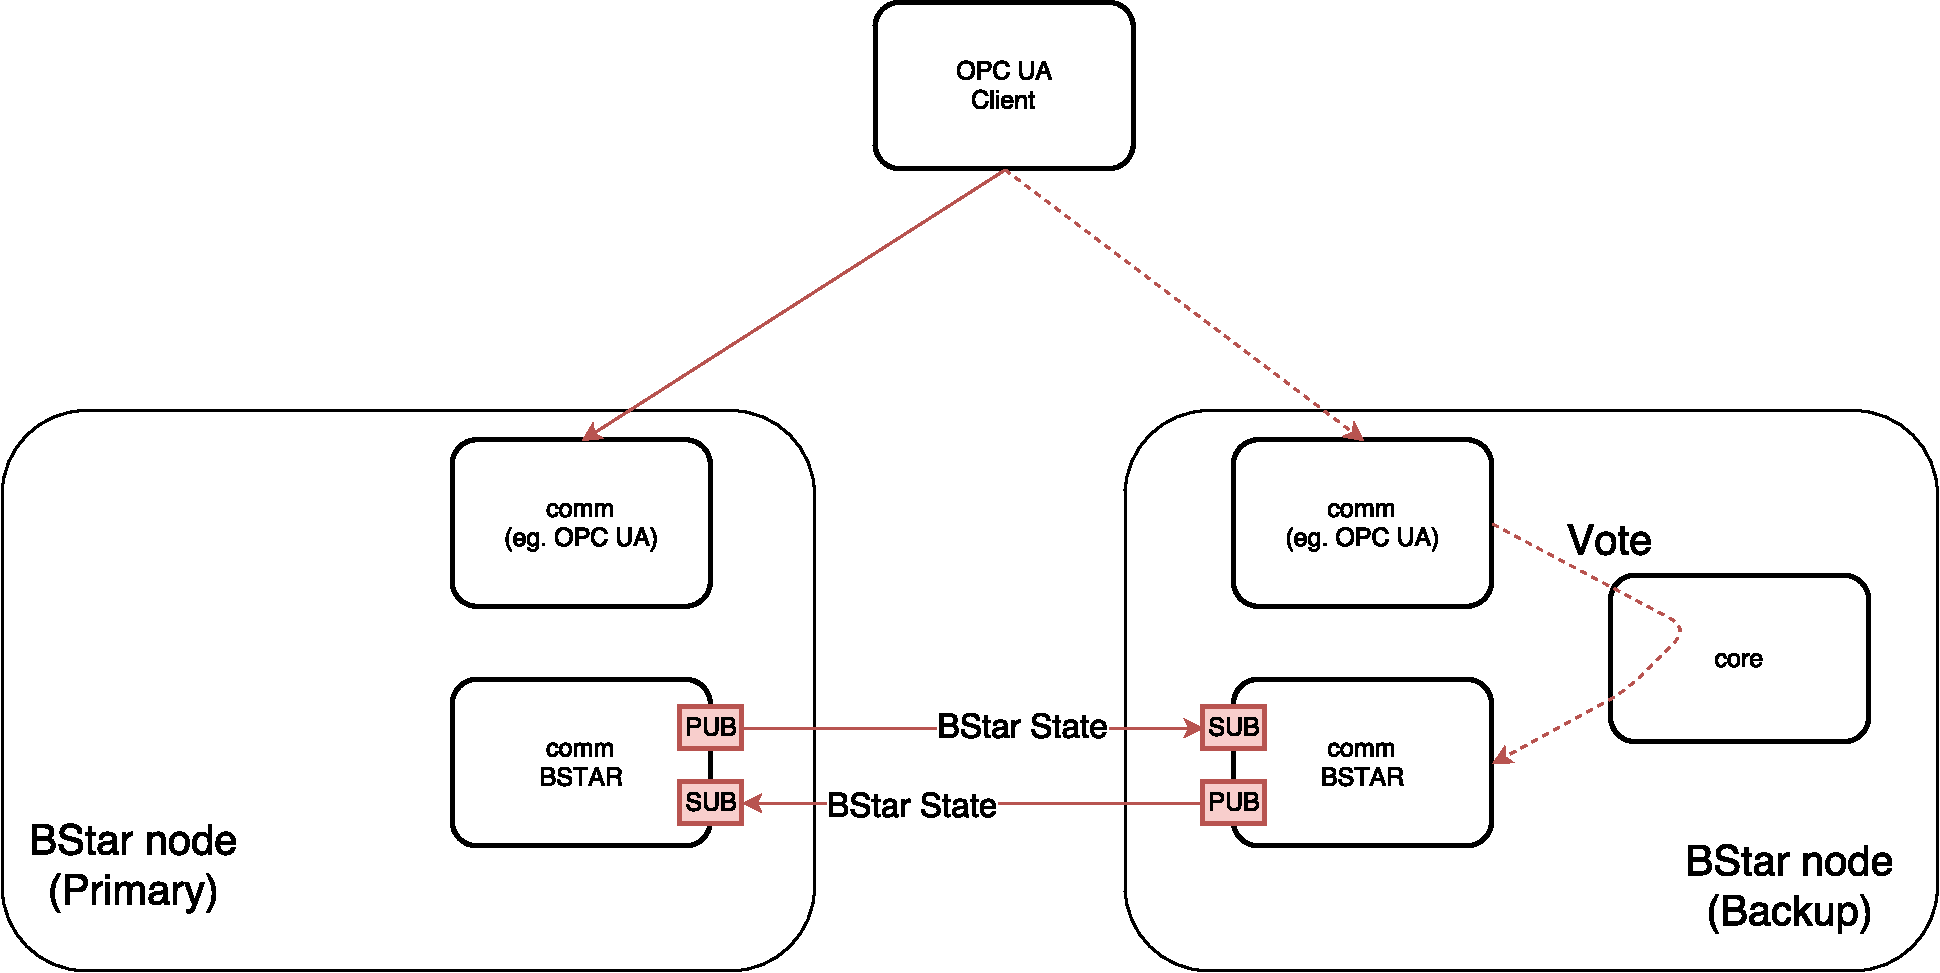
\includegraphics[width=\textwidth]{img/ML-HA_bstar.pdf}
	\caption{Multi level HA setup between a HA pair and a number of client nodes}
	\label{fig:ml-ha}
\end{figure}
% TODO: mention figure in text

%----------------------------------------------------------------------------
\section{Persistence Synchronization}\label{sec:meth:psync}
The persisted data and updates to it, handled by the STORAGE actor, need to
bubble up and collected in the root node.

\subsection{Aspects}
There are multiple aspects involved in persistence synchronization:

\begin{description}
	\item [Delta:]
		How does one get the initial delta of updates since last
		synchronization?

	\item [Updates:]
		Further updates, one-by-one. This is only needed in
		case the solution aims for real-time synchronization.

	\item [HA peer sync:]
		How does the inactive HA peer get updated? Of
		course, this only matters when the supernode is HA pair.
\end{description}

\subsection{Variants}
There are multiple variants to achieve the needed functionality.
% NOTE: Client seems to favor polling.

\subsubsection{Polling only}
The supernode just periodically request persistence
deltas. This would be handled over a DEALER/ROUTER pair of sockets. The nice
thing about this variant is that the subnode only has to do one thing, which is
responding to requests from the supernode(s); it doesn't have to proactively
send any updates after sending the an initial delta.

A big drawback is that the synchronization doesn't happen in real-time. This
doesn't seem to fit well into the overall Roadster architecture, which is
completely event-driven (no polls or "sleeps").

Another drawback is efficiency. This variant will periodically cause the
subnode's database to be searched for all keys. Depending on the size of the
database and the efficiency of searching through keys, this could be a lot of
wasted resources or even cause bottle necks when interacting with the STOR
actor.

In case the supernode is a HA pair, this variant would generate duplicated
traffic. To avoid this, another pair of sockets has to be introduced to
synchronize persistence between a HA pair. This also means designing another
protocol, and more moving parts overall.

Overall, this variant is very simple, but doesn't offer some features we'd
normally expect from a framework like Roadster. The fruits are hanging low;
achieving real-time synchronization and better efficiency is easy.

\subsubsection{PUSH-PULL}
This variant avoids the delays introduced by the polling mechanism of the first variant.

Procedure (for each subnode):
\begin{enumerate}
	\item via a ROUTER/DEALER socket pair:
		\begin{enumerate}
			\item supernode tells subnode its most recent timestamp in an ICANHAZ request
			\item subnode sends delta
			\item supernode receives and processes the complete delta
		\end{enumerate}
	\item subnode sends updates to supernode via PUSH-PULL
	\item during low-traffic times, we can send HUGZ as heartbeats
\end{enumerate}

This seems nice at first, but PUSH socket's send buffer will fill up when the
connection is interrupted.  This isn't bad in and of itself, because when it's
full (and writes start to block), we can just destroy the socket and
reinitialize and start syncing anew (from ICANHAZ) after a certain timeout.
But the problem is that, in case the delta is large, it will inevitably fill
the PUSH socket's send buffer, temporarily reaching its high water mark, which
is part of its normal operation.

So we'd have to introduce logic to recognize whether the PUSH
socket is just temporarily full (e.g. during delta transmission), or
permanently full (e.g. the supernode or the link to it is down).

Another disadvantage is that there needs to be another channel to synchronize
persistence updates to the other HA peer, if there is one. This means another
pair of sockets, another protocol to be designed, and more moving parts
overall.

\subsubsection{PUB/SUB}
This is similar to \gls{CSP}/\gls{CHP}. It's not 100\% reliable, but even with unstable
links, no data loss will occur if the client (the supernode) is able to reconnect within a
specific amount of time. \zmq's default for that amount is 10 seconds. As the
requirements specify, 100\% consistency is not mandatory for the persistent
data.

A possible drawback is that the traffic is duplicated in case the supernode
is a HA pair. However, there are numerous opportunities to mitigate this.

Procedure (for each subnode):
\begin{enumerate}
	\item supernode subscribes to updates from subnode
	\item via a ROUTER/DEALER socket pair:
		\begin{enumerate}
			\item supernode tells subnode its most recent timestamp in an ICANHAZ request
			\item subnode sends delta
			\item supernode receives and processes the complete delta
		\end{enumerate}
	\item supernode starts reading updates, possibly skipping the first few (based on timestamp)
\end{enumerate}

\subsection{Chosen Variant}
We'll most likely go with the PUB-SUB variant, since it's simple and is similar to
what's used for the new \gls{CSP} in conjunction with multi-node \gls{HA}. It provides the best
opportunities to improve efficiency later on.

Its possible performance issues can be ignored right now, as trying to fix them
is arguably considered premature optimization. If this turns out to be an issue
in a productive deployment, like over a cellular network link, a future version
can switch to multicast. \zmq supports PGM, which is a reliable multicast
protocol. (Pragmatic General Multicast, standardized, directly on top of IP,
requires access to raw sockets and thus may require additional privileges) and
EPGM (Encapsulated Pragmatic General Multicast, encapsulated in a series of UDP
datagrams, doesn't require additional privileges, useful in a \zmq-only setup).

If its reliablity turn out to be an issue, one the socket option
\sh{ZMQ_RECOVERY_IVL} can be increased from 10 seconds to, say, 60 seconds, which
gives an unstable link more time to recover before any data loss happens.

TODO: describe reasonable default setting, in case we change ZMQ's default.


\section{Security}\label{sec:meth:security}
Encrypted communication can be achieved using \zmq's transport encryption,
which is completely transparent to the application. It uses the \gls{libsodium}
library to do this, although there's also the possibility to do it using
\gls{tweetnacl} to avoid the additional dependency. The handshake is designed
to be immune against flooding, using encrypted and authenticated cookies, so
the server does not have to allocate any resources before the handshake is
completed.

Server authentication is always done, by specifying the server's public key on
the client side socket.  Client authentication is optional. If done, the server
side socket will talk to an additional socket responsible to authenticate
clients by their public keys. The protocol between these two sockets is called
\gls{ZAP}. Completely abstracting the authentication in another socket allows
any kind of authentication service to be plugged in.

%TODO briefly describe \zmq's security features, what's left for us to decide (key destribution, if at all)\\


\section{OPC UA Interface: High Availability}\label{sec:meth:opc-ua}
TODO This is the optional goal.\\
TODO explain new opportunity for OPC UA HA server\\
TODO describe whatever needs to be described\\


\cite[6.4.2.4 Non-transparent Redundancy, p.~96]{opc-ua:behavior:server-redundancy} describes the exact behavior.

\begin{itemize}
	\item study standard
	\item use Andy's gem
	\item according to Andy, this should be a simple thing
\end{itemize}
